\documentclass{article}
\usepackage[utf8]{inputenc}
\usepackage{graphicx}
\usepackage{soul}

\usepackage{calc}
\usepackage{eso-pic}

\newlength{\PageFrameTopMargin}
\newlength{\PageFrameBottomMargin}
\newlength{\PageFrameLeftMargin}
\newlength{\PageFrameRightMargin}

\setlength{\PageFrameTopMargin}{1cm}
\setlength{\PageFrameBottomMargin}{1cm}
\setlength{\PageFrameLeftMargin}{1cm}
\setlength{\PageFrameRightMargin}{1cm}

\makeatletter

\newlength{\Page@FrameHeight}
\newlength{\Page@FrameWidth}

\AddToShipoutPicture{
  \thinlines
  \setlength{\Page@FrameHeight}{\paperheight-\PageFrameTopMargin-\PageFrameBottomMargin}
  \setlength{\Page@FrameWidth}{\paperwidth-\PageFrameLeftMargin-\PageFrameRightMargin}
  \put(\strip@pt\PageFrameLeftMargin,\strip@pt\PageFrameTopMargin){
    \framebox(\strip@pt\Page@FrameWidth, \strip@pt\Page@FrameHeight){}}}

\makeatother

\title{Computational Mathematics}
\author{Nur Nazifa Sarah Binte Ahmad}
\date{October 2022}

\begin{figure}
    \centering
    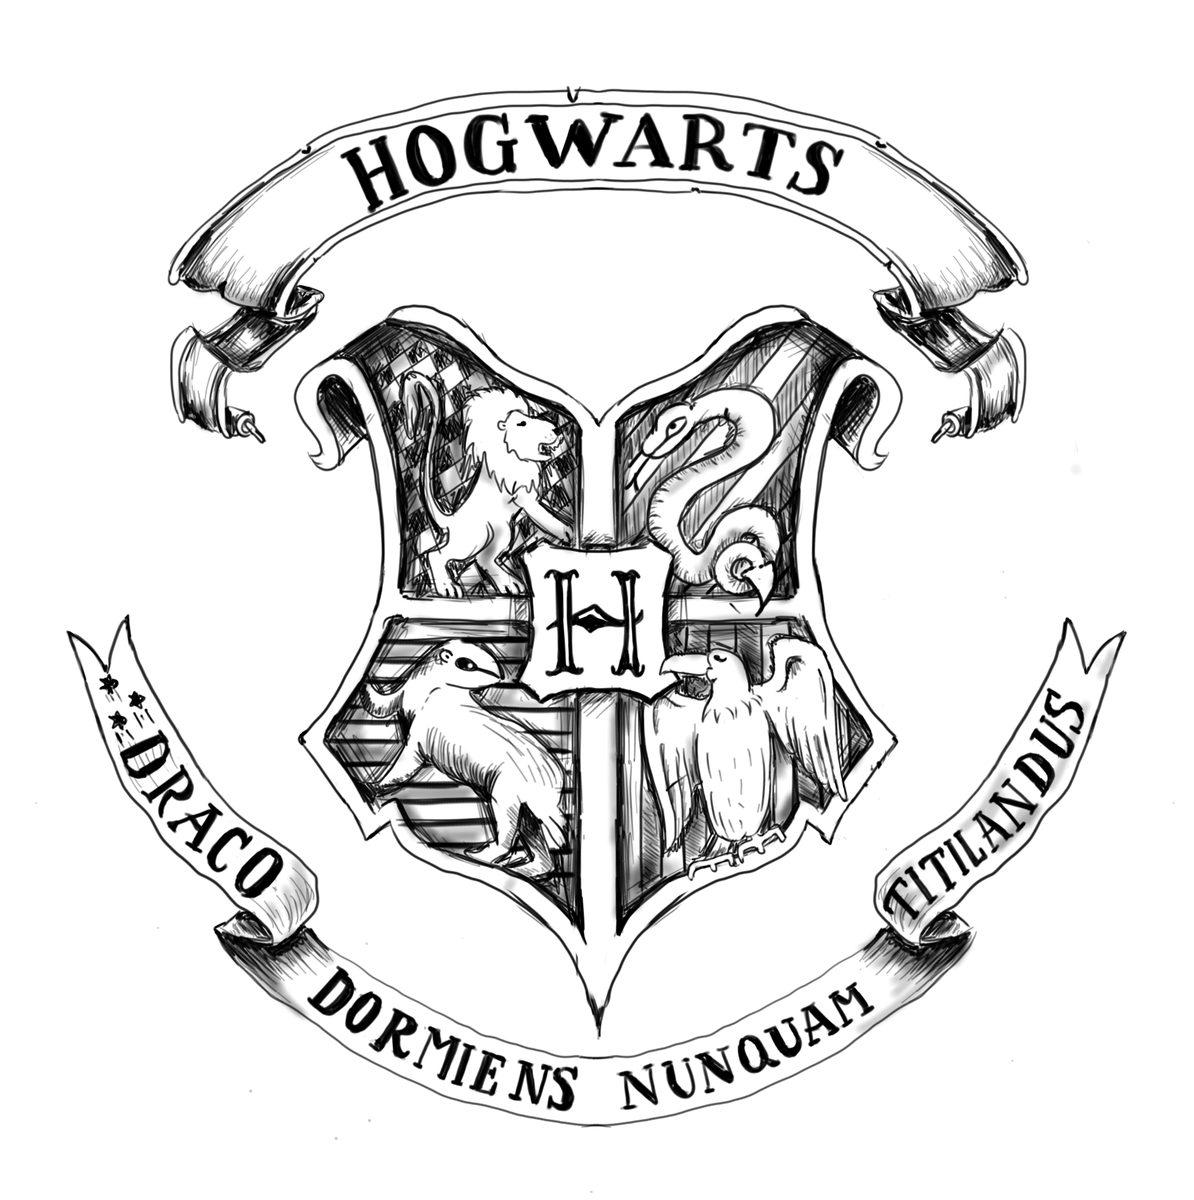
\includegraphics[width = 0.6\textwidth]{Figures/D7iBTImeOxGx28F-Hogwarts-Logo-PNG-Transparent-Images.png}
    \label{fig:my_label}
\end{figure}

\begin{document}
\pagenumbering{Roman}
\maketitle

\newpage

\section*{Contents}
\subsection{Introduction}
\subsection{Base Conversions I}
\subsection{Base Conversions II}
\subsection{Matrix Algebra}
\subsection{Boolean Algebra I}
\subsection{Boolean Algebra II}
\subsection{Matlab: Introduction, Environment and Functions}
\subsection{Matlab: Plotting}
\subsection{Matlab: Programming}
\subsection{Bibliography}

\newpage
\section{Introduction}

This abstract paper was created to present a collection of my calculative interpretations and formulas of the modules above. It is a fairly short overview of my handwritten notes programmed onto the language of LaTeX. As a brief explanation on the language itself, LaTeX is mostly used as a software system for document preparation.

\section{Base Conversions I}
A binary number is a number system that uses bits.

Bit = Binary Digit = 1 bit

Byte = 8 bits
\newline
\newline
\textbf{Decimal Numbering System:}
\newline
$$236$$
$$\downarrow$$
$$(210)$$
$$Conversion\: Algorithm$$
\section*{}
Let us unpack the complete formula for \textbf{236} in the \underline{Decimal Numbering System.}
First, we need to understand the given expression in which both \emph{n} symbolises the individual decimal and conversion respectively. 
$$n*10^n$$
Assign the formula to each decimal number. The number \emph{10} will signify it as a \underline{base of 10.}
$$6*10^0 \to 6 $$
$$\:\:3*10^1 \to 30 $$
$$\:\:\:2*10^2 \to 200 $$
With the given calculations, combine them to obtain the following \underline{answer:}
$$(236)^1^0$$

\newpage
\textbf{Convert Binary Numbers To Decimal Numbers:}
\newline
$$1010$$
$$\downarrow$$
$$(3210)$$
\section*{}
\underline{Convert the given binary number into decimals} by assigning each of it independently. This will be the Binary Numbering System.
$$n*2^n$$
Allocate the formula to each binary number. The number \emph{2} will signify it as a \underline{base of 2,} due to the variable being in binary numbers.
$$0*2^0 \to 0$$
$$1*2^1 \to 2$$
$$0*2^2 \to 0$$
$$1*2^3 \to 8$$
And that is how you convert binary numbers to decimals. With the given calculations, combine them to obtain the following \underline{answer:}
$$(10)^1^0$$
\newline

\textbf{Convert Decimal Numbers To Binary Numbers:}
$$(39)^1^0$$
$$\downarrow$$
$$\underline{2}$$
$$\downarrow$$
$$(100111)^2$$
\newline
Divide the given decimal number into binary using the base of 2. You may review the given formula in the next page for reference.
\newpage
\textbf{Decimal To Binary Formula:}
\newline
\begin{table}[h!]
    \centering
    \begin{tabular}{|c|c|c|}
        \textbf{Divisor} & \textbf{Quotient} & \textbf{Remainder} \\
        2 & 39 & X \\
        2 & 19 & 1 \\
        2 & 9 & 1 \\
        2 & 4 & 1 \\
        2 & 2 & 0 \\
        2 & 1 & 0 \\
        
    \end{tabular}
    \caption{Example}
    \label{tab:my_label}
\end{table}
$$\downarrow$$
\begin{table}[h!]
    \centering
    \begin{tabular}{|c|c|c|}
        \textbf{Divisor} & \textbf{Quotient} & \textbf{Remainder} \\
        2 & 39 & X \\
        2 & 19 & \underline{1} \\
        2 & 9 & \underline{1} \\
        2 & 4 & \underline{1} \\
        2 & 2 & \underline{0} \\
        2 & \underline{1} & \underline{0} \\
        
    \end{tabular}
    \caption{Example}
    \label{tab:my_label}
\end{table}
\newline
As depicted in the tables above, we can now determine the solution by listing down the final quotient of 1 and all of the remainders in order. This will provide you with binary numbers that are equivalent to the initial decimals. \underline{Hence, the answer is as follows:}
\newline
$$(100111)^2 = 0010 0111$$
\newline
$$Summary$$
$$\downarrow$$
$$(39)^1^0$$
$$\downarrow$$
$$(100111)^2$$
$$\downarrow$$
$$00100111$$

\newpage

\textbf{Binary To Decimals:}
\newline
$$\underline{01011011}$$
$$\downarrow$$
$$(76543210)$$
$$\downarrow$$
$$1*2^0=1$$
$$1*2^1=2$$
$$0*2^2=0$$
$$1*2^3=8$$
$$1*2^4=16$$
$$0*2^5=0$$
$$1*2^6=64$$
$$0*2^7=0$$
$$\downarrow$$
$$0+64+0=16+8+0+2+1=(91)^1^0$$
\newline
$$\textbf{OR}$$
\newline
$$\underline{10101100}$$
$$\downarrow$$
$$(76543210)$$
$$\downarrow$$
$$1*(2^7)+0*(2^6)+1*(2^5)+0*(2^4)+1*(2^3)+1*(2^2)+0*(2^1)+0*(2^0)$$
$$\downarrow$$
$$(172)^1^0$$

\newpage
\textbf{Decimals To Binary:}
\begin{table}[h!]
    \centering
    \begin{tabular}{|c|c|c|}
        \textbf{Divisor} & \textbf{Quotient} & \textbf{Remainder} \\
        2 & 328 & X \\
        2 & 164 & 0 \\
        2 & 82 & 0 \\
        2 & 41 & 0 \\
        2 & 20 & 1 \\
        2 & 10 & 0 \\
        2 & 5 & 0 \\
        2 & 2 & 1 \\
        2 & 1 & 0 \\
        
    \end{tabular}
    \caption{Example}
    \label{tab:my_label}
\end{table}
$$\downarrow$$
\begin{table}[h!]
    \centering
    \begin{tabular}{|c|c|c|}
        \textbf{Divisor} & \textbf{Quotient} & \textbf{Remainder} \\
        2 & 328 & X \\
        2 & 164 & \underline{0} \\
        2 & 82 & \underline{0} \\
        2 & 41 & \underline{0} \\
        2 & 20 & \underline{1} \\
        2 & 10 & \underline{0} \\
        2 & 5 & \underline{0} \\
        2 & 2 & \underline{1} \\
        2 & \underline{1} & \underline{0} \\
        
    \end{tabular}
    \caption{Example}
    \label{tab:my_label}
\end{table}
$$\downarrow$$
$$(101001000)^2$$
$$\downarrow$$
$$000101001000$$
$$\downarrow$$
$$Answer$$

\newpage
\textbf{Decimals To Binary:}
\begin{table}[h!]
    \centering
    \begin{tabular}{|c|c|c|}
        \textbf{Divisor} & \textbf{Quotient} & \textbf{Remainder} \\
        2 & 733 & X \\
        2 & 366 & 1 \\
        2 & 183 & 0  \\
        2 & 91 & 1 \\
        2 & 45 & 1 \\
        2 & 22 & 1 \\
        2 & 11 & 0 \\
        2 & 5 & 1 \\
        2 & 2 & 1 \\
        2 & 1 & 0 \\
        
    \end{tabular}
    \caption{Example}
    \label{tab:my_label}
\end{table}
$$\downarrow$$
\begin{table}[h!]
    \centering
    \begin{tabular}{|c|c|c|}
        \textbf{Divisor} & \textbf{Quotient} & \textbf{Remainder} \\
        2 & 733 & X \\
        2 & 366 & \underline{1} \\
        2 & 183 & \underline{0}  \\
        2 & 91 & \underline{1} \\
        2 & 45 & \underline{1} \\
        2 & 22 & \underline{1} \\
        2 & 11 & \underline{0} \\
        2 & 5 & \underline{1} \\
        2 & 2 & \underline{1} \\
        2 & \underline{1} & \underline{0} \\
        
    \end{tabular}
    \caption{Example}
    \label{tab:my_label}
\end{table}
$$\downarrow$$
$$(1011011101)^2$$
$$\downarrow$$
$$001011011101$$
$$\downarrow$$
$$Answer$$

\newpage
\newline
\textbf{Convert Octal Numbers To Decimal Numbers:}
\section*{}
$$(275)^8$$
$$\downarrow$$
$$2=(421), 7=(421), 5=(421)$$
\section*{}
Octal numbers are prominently known to be in base 8 and in 3 bits for each octal number. In order to obtain the solution, we will need to allocate each octal to 4, 2 and 1 to retrieve the following:
$$(275)^8$$
$$\downarrow$$
$$010, 111, 101$$
$$\downarrow$$
$$(010111101)^2$$
$$\downarrow$$
$$000010111101$$
\newline
\textbf{Convert Hexadecimal Numbers To Decimal Numbers:}
$$1AC$$
$$\downarrow$$
$$(210)$$
$$conversion$$
$$\downarrow$$
$$base=16$$
$$\downarrow$$
$$Hex+Table$$
$$\downarrow$$
$$(1*16^2)+(10*16^1)+(12*16^0)$$
$$\downarrow$$
$$\underline{428}$$
\newpage
\textbf{Convert Decimal Numbers To Hexadecimal Numbers:}
\begin{table}[h!]
    \centering
    \begin{tabular}{|c|c|c|}
        \textbf{Divisor} & \textbf{Quotient} & \textbf{Remainder} \\
        16 & 335 & X \\
        16 & 20 & 15 \\
        16 & 1 & 4  \\
        
    \end{tabular}
    \caption{Example}
    \label{tab:my_label}
\end{table}
\textbf{Convert Hexadecimal Numbers To Binary Numbers:}
$$1AC$$
$$\downarrow$$
$$(0001), (1010), (1100)$$
$$conversion$$
$$\downarrow$$
$$multiples-of-8$$
$$\downarrow$$
$$0000,0001,1010,1100$$
$$\downarrow$$
$$hence$$
$$\downarrow$$
$$0000000110101100$$
$$\downarrow$$
$$Answer$$

\newpage
\section{Base Conversion II}

To add binary numbers, we need to understand that the arithmetic solution will require that we calculate them in base 2.
$$1=true$$
$$0=false$$

\textbf{Adding Binary Numbers:}
\begin{table}[h!]
    \centering
    \begin{tabular}{|c|}
    \hline
        \textbf{Addition} \\
        0101  \\
        +  \\
        0011   \\
        \hline
               \textbf{Answer} \\
        ?  \\ 
        \hline
    \end{tabular}
    \label{tab:my_label}
\end{table}
$$\downarrow$$
\begin{table}[h!]
    \centering
    \begin{tabular}{|c|}
    \hline
        \textbf{Addition} \\
        0^11^10^11  \\
        +  \\
        0011   \\
        \hline
               \textbf{Answer} \\
        1000  \\ 
        \hline
    \end{tabular}
    \label{tab:my_label}
\end{table}
\newline
\newline
To make it more simpler, in binary addition, 1+1 will provide you with binary number 0. While 1+0, or 0+1, will provide you with binary number 1. And finally, 0+0 will provide you with binary number 0.
\section*{}
$$Answer$$
$$\downarrow$$
$$1000$$
\newpage
\textbf{Subtracting Binary Numbers:}
\newline
\newline
For binary subtraction, we will need to borrow if the minuend is not enough to be deducted from during calculating.
\newline
\begin{table}[h!]
    \centering
    \begin{tabular}{|c|}
    \hline
        \textbf{Addition} \\
        0101  \\
        -  \\
        0011   \\
        \hline
               \textbf{Answer} \\
        ?  \\ 
        \hline
    \end{tabular}
    \label{tab:my_label}
\end{table}
$$\downarrow$$
\begin{table}[h!]
    \centering
    \begin{tabular}{|c|}
    \hline
        \textbf{Addition} \\
        0101  \\
        -  \\
        0011   \\
        \hline
               \textbf{Answer} \\
        10  \\ 
        \hline
    \end{tabular}
    \label{tab:my_label}
\end{table}
\newline
\newline
Below is the final workings for the subtraction:
\newline
\newline
\centerline{01\st{0}^1^01 = 0011}
\section*{}
Borrow the second binary from the left for the third binary. This will cause the borrowed binary to be 10. Hence, 10 turned to 1, once subtracted with 1, equates to 1.

$$0011-0011$$

\newpage
\textbf{Multiplying Binary Numbers:}
\newline
\newline
\begin{table}[h!]
    \centering
    \begin{tabular}{|c|}
    \hline
        \textbf{Multiply} \\
        0101  \\
        x  \\
        0011   \\
        \hline
               \textbf{Answer} \\
        ?  \\ 
        \hline
    \end{tabular}
    \label{tab:my_label}
\end{table}
$$\downarrow$$
$$0101$$
$$\downarrow$$
$$add$$
$$\downarrow$$
$$01010$$
$$\downarrow$$
$$answer$$
$$\downarrow$$
$$01111$$
$$\downarrow$$
\begin{table}[h!]
    \centering
    \begin{tabular}{|c|}
    \hline
        \textbf{Multiply} \\
        0101  \\
        x  \\
        0011   \\
        \hline
               \textbf{Answer} \\
        01111  \\ 
        \hline
    \end{tabular}
    \label{tab:my_label}
\end{table}
\section*{}
We can obtain the answer from the formula given above. Addition for binaries is simple, as long we take note of placing 0's to the right hand side, based on the binary number sequence.
\newpage
\textbf{Adding Octal Numbers:}
\subsection*{}

When it comes to adding Octals, we must carry over the remainder if its adds up to the number 8. This is due to the fact that Octals are in base 8.
\newline
\begin{table}[h!]
    \centering
    \begin{tabular}{|c|}
    \hline
        \textbf{Addition} \\
        135  \\
        +  \\
        26   \\
        \hline
               \textbf{Answer} \\
        ?  \\ 
        \hline
    \end{tabular}
    \label{tab:my_label}
\end{table}
$$\downarrow$$
\begin{table}[h!]
    \centering
    \begin{tabular}{|c|c|}
    \hline
        \textbf{Addition} & \textbf{Remainder}  \\
        135 & 5+6=R1 \\
        +  & R1+3+2 \\
        26 & 1 \\
        \hline
               \textbf{Equates} & \textbf{Answer}\\
        163 & 163 \\ 
        \hline
    \end{tabular}
    \label{tab:my_label}
\end{table}
\newline
To obtain the answer, we need to add 5+6=3 with a remainder of 1 due it in being in base 8, or Octals. Hence, 11-8=3, meaning the remainder will be 1. Afterwards, combine 3+2 with the remainder of 1 in order to retrieve 3. The answer will then be 163.
$$\downarrow$$
$$135+26$$
$$\downarrow$$
$$answer$$
$$\downarrow$$
$$163$$
\newpage
\textbf{Adding Hexadecimal Numbers:}
\section*{}
We can add the Hexadecimal Numbers by converting it into decimals using the hexadecimal chart.
\newline
$$1A+2C$$
$$\downarrow$$
$$1(10)+2(12)$$
\newline
We must first conclude that 10+12=22 will provide us with 16 instead, as it is in base 16. Afterwards, carry over the number 1 from 16, so that we may add it with 1 and 2. Hence, 1+1+2 will give us the number 4. Since 4 is still a part of base 16, we will consider this number in the solution. We can then determine that the answer is:
$$46$$
$$\downarrow$$
$$answer$$
\newline
\section*{}
\begin{table}[h!]
    \centering
    \begin{tabular}{|c|}
    \hline
        \textbf{End of Chapter for Base Conversions} \\
        \hline

        \hline
    \end{tabular}
    \label{tab:my_label}
\end{table}
\newpage
\section{Matrix Algebra}
\newline
In Matrices, each item found in a matrix is referred to as an element. And the collection of numbers in rows and columns can be 
\end{document}





